\documentclass{standalone}
\usepackage{tikz}
\begin{document}
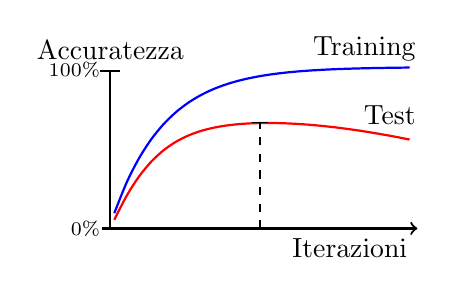
\begin{tikzpicture}
    \draw[thick, ->](-0.1,0)--++(4,0)node[below left]{Iterazioni};
    \draw[-|, thick](0,0)node[left]{\scriptsize $0\%$}--++(0,2.01)node[left]{\scriptsize $100\%$}node[above]{Accuratezza};
    \draw[thick, blue]plot[smooth, domain=0.05:3.8](\x, {2-2*e^(-\x*1.5)+0.05});
    \draw[thick, red]plot[smooth, domain=0.05:3.8](\x, {1.5*sin((180*\x*1.5*e^(-0.5*\x))/pi)});
    \draw(4,2)node[above left]{Training};
    \draw(4,1.2)node[above left]{Test};
    \draw[dashed, -|](1.9,0)--++(0,1.35);
\end{tikzpicture}
\end{document}